\documentclass[a4paper]{article}
\usepackage[utf8x]{inputenc}
\usepackage[T1,T2A]{fontenc}
\usepackage[russian]{babel}
\usepackage{hyperref}
\usepackage{indentfirst}
\usepackage{listings}
\usepackage{color}
\usepackage{here}
\usepackage{array}
\usepackage{multirow}
\usepackage{graphicx}

\usepackage{caption}
\renewcommand{\lstlistingname}{Программа} % заголовок листингов кода

\usepackage{amssymb,amsfonts,amsmath} % Математика
\numberwithin{equation}{section} % Формула вида секция.номер

\usepackage{listings}
\lstset{ %
extendedchars=\true,
keepspaces=true,
language=C,						% choose the language of the code
basicstyle=\footnotesize,		% the size of the fonts that are used for the code
numbers=left,					% where to put the line-numbers
numberstyle=\footnotesize,		% the size of the fonts that are used for the line-numbers
stepnumber=1,					% the step between two line-numbers. If it is 1 each line will be numbered
numbersep=5pt,					% how far the line-numbers are from the code
backgroundcolor=\color{white},	% choose the background color. You must add \usepackage{color}
showspaces=false				% show spaces adding particular underscores
showstringspaces=false,			% underline spaces within strings
showtabs=false,					% show tabs within strings adding particular underscores
frame=single,           		% adds a frame around the code
tabsize=2,						% sets default tabsize to 2 spaces
captionpos=b,					% sets the caption-position to bottom
breaklines=true,				% sets automatic line breaking
breakatwhitespace=false,		% sets if automatic breaks should only happen at whitespace
escapeinside={\%*}{*)},			% if you want to add a comment within your code
postbreak=\raisebox{0ex}[0ex][0ex]{\ensuremath{\color{red}\hookrightarrow\space}},
texcl=true,
}

\usepackage[left=2cm,right=2cm,
top=2cm,bottom=2cm,bindingoffset=0cm]{geometry}


\begin{document} % начало документа
\raggedbottom
%\begin{titlepage}	% начало титульной страницы

	\begin{center}		% выравнивание по центру

		\large Санкт-Петербургский Политехнический Университет Петра Великого\\
		\large Институт компьютерных наук и технологий \\
		\large Кафедра компьютерных систем и программных технологий\\[6cm]
		% название института, затем отступ 6см
		
		\huge Название предмета\\[0.5cm] % название работы, затем отступ 0,5см
		\large Отчет по лабораторной работе №1\\[0.1cm]
		\large Тема работы\\[5cm]

	\end{center}


	\begin{flushright} % выравнивание по правому краю
		\begin{minipage}{0.25\textwidth} % врезка в половину ширины текста
			\begin{flushleft} % выровнять её содержимое по левому краю

				\large\textbf{Работу выполнил:}\\
				\large Петров В.Д.\\
				\large {Группа:} 43501/4\\
				
				\large \textbf{Преподаватель:}\\
				\large Ицыксон В.М.

			\end{flushleft}
		\end{minipage}
	\end{flushright}
	
	\vfill % заполнить всё доступное ниже пространство

	\begin{center}
	\large Санкт-Петербург\\
	\large \the\year % вывести дату
	\end{center} % закончить выравнивание по центру

\thispagestyle{empty} % не нумеровать страницу
\end{titlepage} % конец титульной страницы

\vfill % заполнить всё доступное ниже пространство



% Содержание
%\tableofcontents
%\newpage
\title{Обзор алгоритмов стереозрения для применения в мобильной робототехнике}
\author{Пантелеев М.}
\institute{Санкт-Петербургский Политехнический Университет Петра Великого
\email{panteleev.md@edu.spbstu.ru}}
\maketitle

\begin{abstract}
	% TODO: дополнить  
	В этой статье приводится обзор алгоритмов, связанных с сопоставлением двух изображений.
\end{abstract}

\section{Введение}
Получение трёхмерной структуры пространства по стереоснимкам - это задача, подходы к которой начали искать очень давно. И хотя 
множество подходов к решению было найдено, исследователи продолжают работу над более эффективными алгоритмами. В силу дешевизны (относительно других сенсоров,
позволяющих получить объёмную информацию о пространстве) и универсальности камер, на подобные методики есть большой спрос со стороны 
таких областей как автономный транспорт и мобильная робототехника. 					% TODO: уточнить
Эти области весьма требовательны к точности результатов и скорости работы алгоритмов, так как устройства должны принимать оперативные решения на основе 
данных о внешнем мире, а мощности бортовых вычислителей весьма ограничены. Именно эти качества находятся в фокусе современных исследований, поэтому в этой 
работе также будет уделено внимание возможности того или иного алгоритма работать в реальном времени. Эта возможность характеризуется частотой, с которой 
алгоритм просчитывает карты глубины. Очевидно, что фактическое значение частоты кадров сильно зависит от используемого вычислителя и разрешения камер, поэтому 
для теоретического сравнения больше подходит вычислительная сложность алгоритма. 

% TODO: occlusion : заслонение -> затенение / окклюзия
При этом в стереозрении есть ряд проблем и ограничений, которые осложняют получение надёжной и полной информации по снимкам. Часть этих проблем 
связана с недостатками самого способа получения изображений (заслонение), другая часть - с особенностями отображения некоторых поверхностей на 
двумерных снимках (наклонные плоскости или слаботекстурированные области). Снижение влияния этих 
ограничений на результат путём создания новых алгоритмов или модификации существующих является второй важной целью исследователей. 

Остальная часть статьи организована следующим образом: в продолжении этой секции рассмотрен базовый принцип стереозрения, секция \ref{matching} описывает 
самые популярные подходы к построению карт расхождения и их применимость для получения результатов в реальном времени, в секции \ref{conclusion} представлены выводы. 

\subsection{Принцип стереозрения}
Несмотря на существование разных алгоритмов стереозрения, все они реализуют общий принцип. Задача стереозрения 
 состоит в использовании двух или более камер для получения данных о дальности до объектов в кадре. 

Как правило, система стереозрения состоит из двух камер, наблюдающих сцену с разных точек, как изображено на рисунке \ref{pic:epipol} \cite{Hartley2004}. 
Фундаментальная основа принципа заключается в предположении, что каждой точке в пространстве соответствует уникальная пара пикселей на снимках с двух камер.  

При этом к камерам предъявляются некоторые требования \cite{rusoverview}:   % не уверен, что это надо цитировать
\begin{itemize}
	\item Камеры откалиброваны. Это значит, что известны внутренние (оптические) и внешние (расположение камер в пространстве) параметры камер. 
	\item Ректификация. Подразумевает выравнивание изображения с обеих камер по строкам.  % Мб подробнее расписать  
	\item Ламбертовость поверхностей. Означает независимость освещения поверхности от угла зрения. 
\end{itemize}

\begin{figure}[H]
	\begin{center}
		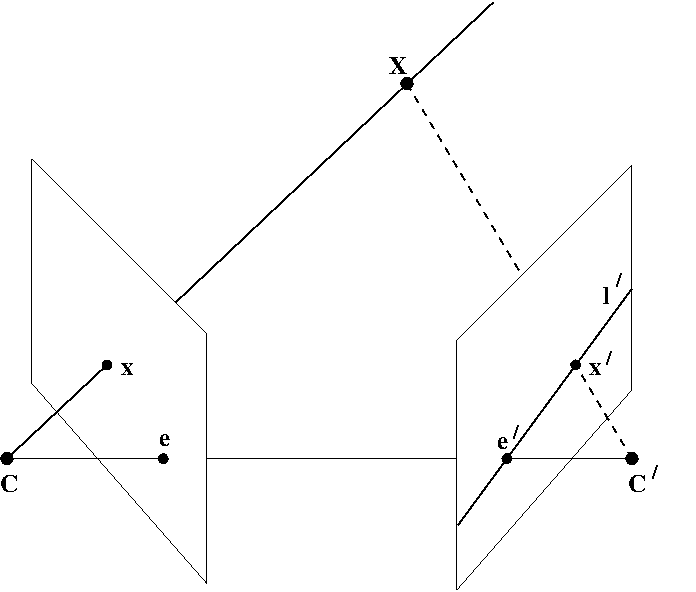
\includegraphics[scale=0.5]{pics/epipolar geometry.png}
		\caption{Эпиполярная геометрия} 
		\label{pic:epipol} % название для ссылок внутри кода
	\end{center}
\end{figure}

Таким образом, соблюдение указанных выше требований позволяет использовать следующий геометрический принцип. При наличии двух камеры, как изображено 
на рисунке \ref{pic:epipol}, где $C$ — центр первой камеры, $C'$ — центр второй камеры, точка пространства $X$  
проецируется в $x$ на плоскость изображения левой камеры и в $x'$ на плоскость изображения правой камеры. Прообразом точки $x$ на изображении левой 
камеры является луч $xX$. Этот луч проецируется на плоскость второй камеры в прямую $l'$, называемую эпиполярной линией. Образ точки $X$ на плоскости 
изображения второй камеры обязательно лежит на эпиполярной линии $l'$.

В результате каждой точке $x$ на изображении левой камеры соответствует эпиполярная линия $l'$ на изображении правой камеры. При этом соответствие для $x$ на 
изображении правой камеры может лежать только на соответствующей эпиполярной линии. Аналогично, каждой точке $x'$ на правом изображении соответствует 
эпиполярная линия $l$ на левом.

Далее с помощью точек $x$ и $x'$ возможно посчитать смещения каждого пикселя одного изображения относительно другого, что даёт карту смещений (disparity map). 
Очевидно, что смещения будут подсчитаны только для точек, видимых обеими камерами. Карта смещений же приводится далее либо к облаку точек, либо к карте глубины. 
Пример такой карты представлен на рисунке \ref{pic:depth} \cite{lipson2021raft}. 

\begin{figure}[H]
	\begin{center}
		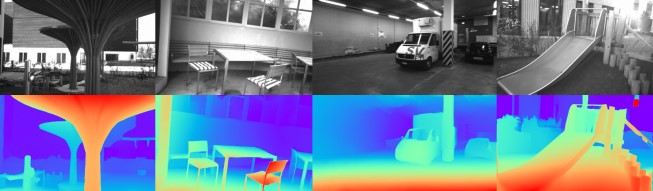
\includegraphics[scale=0.7]{pics/exmpl.jpg}
		\caption{Примеры результата работы} 
		\label{pic:depth} % название для ссылок внутри кода
	\end{center}
\end{figure}

На практике работу большинства алгоритмов можно разделить на 3 этапа: получение изображений, поиск соответствий и восстановление информации о глубине. Это позволяет
организовать классификацию алгоритмов на основе подходов к каждому из этих этапов. В этой статье будут рассмотрены в основном лишь методы поиска соответствий на изображениях. 

Восстановление заключается в расчёте глубины по известным внешним параметрам камер. Глубина каждой точки $X$, воспринимаемой двумя камерами 
с оптическими центрами $C$ и $C'$, определяется проекциями $x$, $x'$ этой точки на каждый кадр. Тогда значение глубины можно найти по уравнению \ref{eq:Z}, указанному ниже. 
\begin{equation}	
	Z = f{T \over d},
	\label{eq:Z}
\end{equation}
где T - расстояние между $C$ и $C'$;
    d - смещение,  {d = x - x'};
	f - фокусное расстояние камеры.

Получение изображений обычно осуществляется с использованием двух синхронизированных камер. Однако есть работы \cite{singlecamrev,singlecam}, которые 
решают эту задачу с использованием лишь одной камеры совместно с системой линз и зеркал, но принцип их функционирования по своей сути 
 симулирует двухкамерную реализацию. 
 
 Другой вектор работ направлен на получение информации о глубине по снимках, сделанным с помощью камер со сверхшироким 
 углом обзора, так как они часто встречаются в мобильных роботах \cite{omnifisheye,roxas2019realtime}, но существующие работы пока не могут обеспечить результаты, 
 сравнимые с традиционными камерами без существенных вычислительных затрат. 

\section{Поиск соответствий}
\label{matching}
Как было ранее сказано, поиск соответствий можно выполнять широким набором методов. Цель каждого метода - постараться найти для каждого пикселя одной картинки 
соответствующий ему пиксель на второй. Достичь этого можно двумя подходами в зависимости от накладываемых на зону поиска соответствий ограничений.  При подсчёте 
расхождений лишь в небольшой окрестности (окне) вокруг интересующего нас пикселя мы говорим о локальных методах, эти методы  используют небольшое количество 
информации и относительно быстродействены. Локальные методы в свою очередь принято делить на три категории: сопоставление блоков, градиентные методы и 
сопоставление признаков. 		% TODO: я не особо следую этому, мб переписать

Глобальные методы же обрабатывают целый ряд пикселей или всё изображение целиком. Они не так чувствительны к локальным дефектам, мешающим процессу поиска соответствий 
(например, заслонение), но при этом имеют куда большую вычислительную сложность. Одними из самых популярных подходов в этой группе методов являются динамическое программирование \cite{dynamic_prog},
алгоритм разреза графа и ... % TODO: уточнить.   	 

\subsection{Сопоставление блоков}
Block Matching - это локальный метод, который заключается в оценке расхождения в точке на одной картинке с помощью сравнения небольшой области вокруг этой точки с такими же областями 
на другой \cite{}. Благодаря выпрямлению (ректификации) поиск соответствующей области на другой картинке ограничивается одним измерением. По этому измерению (как правило, строке) 
считается одна из доступных метрик, и регион с наименьшим её значением считается искомым. Существует целый набор метрик, часто используемых в этом методе. 

Для отдельных пар пикселей можно рассчитывать абсолютную разность (AD) или квадратичную разность (SD), выраженную через интенсивности:
\begin{equation}
	AD(x, y, d) = |I_l(x,y) - I_r(x+d, y)|,			
	\label{eq:AD}
\end{equation}
где $(x, y)$ - координаты первого пикселя; $d$ - сдвиг по оси x между двумя пикселями (смещение); $I$ - интенсивность данного пикселя. Обычно $I_l$ обозначают опорное изображение, а $I_r$ - 
целевое. Абсолютная разность - простейшая метрика, за счёт чего до сих пор используется в многих алгоритмах, от которых требуется производительность в реальном времени. 

Для квадратичной разности 
\begin{equation}
	SD(x, y, d) = |I_l(x,y) - I_r(x+d, y)|^2.		
	\label{eq:SD}
\end{equation}

На основании этих метрик были выведены более точные и сложные, такие как сумма квадратичных разностей (SSD) и сумма абсолютных разностей (SAD). Они применяют описанный выше принцип для целого 
окна пикселей вокруг исследуемого.  Благодаря всё ещё достаточно высокой скорости работы эти метрики позволяют повышать качество итоговой карты смещений за счёт варьирования размера окна и 
дополнительных проходов по изображениям \cite{twosizewindow} 

Также применяется нормированная кросс-корреляция (NCC) - стандартный статистический метод для поиска соответствий с шаблоном, который записывается для случая поиска соответствий пикселей 
согласно уравнению \ref{equ:NCC}.

\begin{equation}
	NCC(x, y) = \frac{ \sum_{x, y}^{} (I_l(x, y) - \overline{I_l} )^2 * ( I_r(x + d, y) - \overline{I_r} )^2   }{ \sqrt{ \sum_{x, y}^{} (I_l(x, y) - \overline{I_l} )^2 * ( I_r(x + d, y) - \overline{I_r} )^2 }  }, 
	\label{equ:NCC}
\end{equation}

где $\overline{I_l}$ и $\overline{I_r}$ - средние интенсивности соответствующих изображений. Эта метрика устойчива к перепадам яркости и контрастности изображения благодаря нормализации \cite{ncceval}, 
но требует выполнения значительно большего числа арифметических операций для своего подсчёта. 

Таким образом, почти любой алгоритм сопоставления блоков позволяет получать относительно быстрые результаты сам по себе, но точность остаётся маленькой и чувствительной к различным условиям освещения. 

\subsection{Сопоставление признаков}
Довольно распространёнными являются методы, основанные на использовании характерных точек - методы SIFT \cite{sift}, SURF \cite{surf} 
и методы, основанные на детекторах Харриса и других. Различным способам поиска этих характерных точек посвящено немало статей. 

Суть методов, относящихся к этой группе, заключается в выделении на снимках характерных точек: углов и точек смены контраста. Далее 
для найденных точек считается дискриптор - вектор, являющийся численной характеристикой окрестности характерной точки. Таким образом,
установление соответствий сводится к сравнению численных величин этих векторов. 

Новые работы в этой области продолжают публиковаться. Так был предложен метод на основе SIFT, использующий самоорганизующиеся карт для 	% TODO: почитпть про эти карты
достижения более высокой производительности \cite{modsift}. Работа Liu и других \cite{ekstrand2015high} же опирается на использование комбинации из сегментации 
изображения и обнаружения границ в качестве метрики поиска совпадений. Такая реализация работает быстро, но точность результатов по-прежнему остаётся
невысокой, особенно в областях прерывистости. % discontinuity

Метод менее чувствителен к перекрытиям и слаботекстурированным областям, 
но, к сожалению, плотность точек, для которых возможно подсчитать глубину, получается относительно низкой, что привело к снижению интереса 
к этой группе методов.

% ГЛОБАЛЬНЫЕ
\subsection{Методы динамического программирования}
Методы, основанные на динамическом программировании, являются одними из самых часто используемых среди глобальных подходов.  
В случае с поиском совпадений на изображениях это означает введение новой конструкции - DSI (disparity space image). Строится она следующим образом: 
выбираются $i$-ые строки левого и правого изображения (они должны быть ректифицированы), далее одна строка постепенно "сдвигается" относительно другой и
на каждом этапе разность между совпадающими пикселями записывается в DSI, который в итоге содержит в себе разницы каждого пикселя с каждым для всех попарных
 рядов исходных изображений. Строки DSI, соответствующие заведомо невозможным значениям (например, расхождения больше максимально допустимых или пиксель на левом изображении 
 находится левее соответствующего ему на правом) отбрасываются. 
Рисунок \ref{pic:DSI} \cite{DSI} иллюстрирует этот принцип. 
\begin{figure}[H]
	\begin{center}
		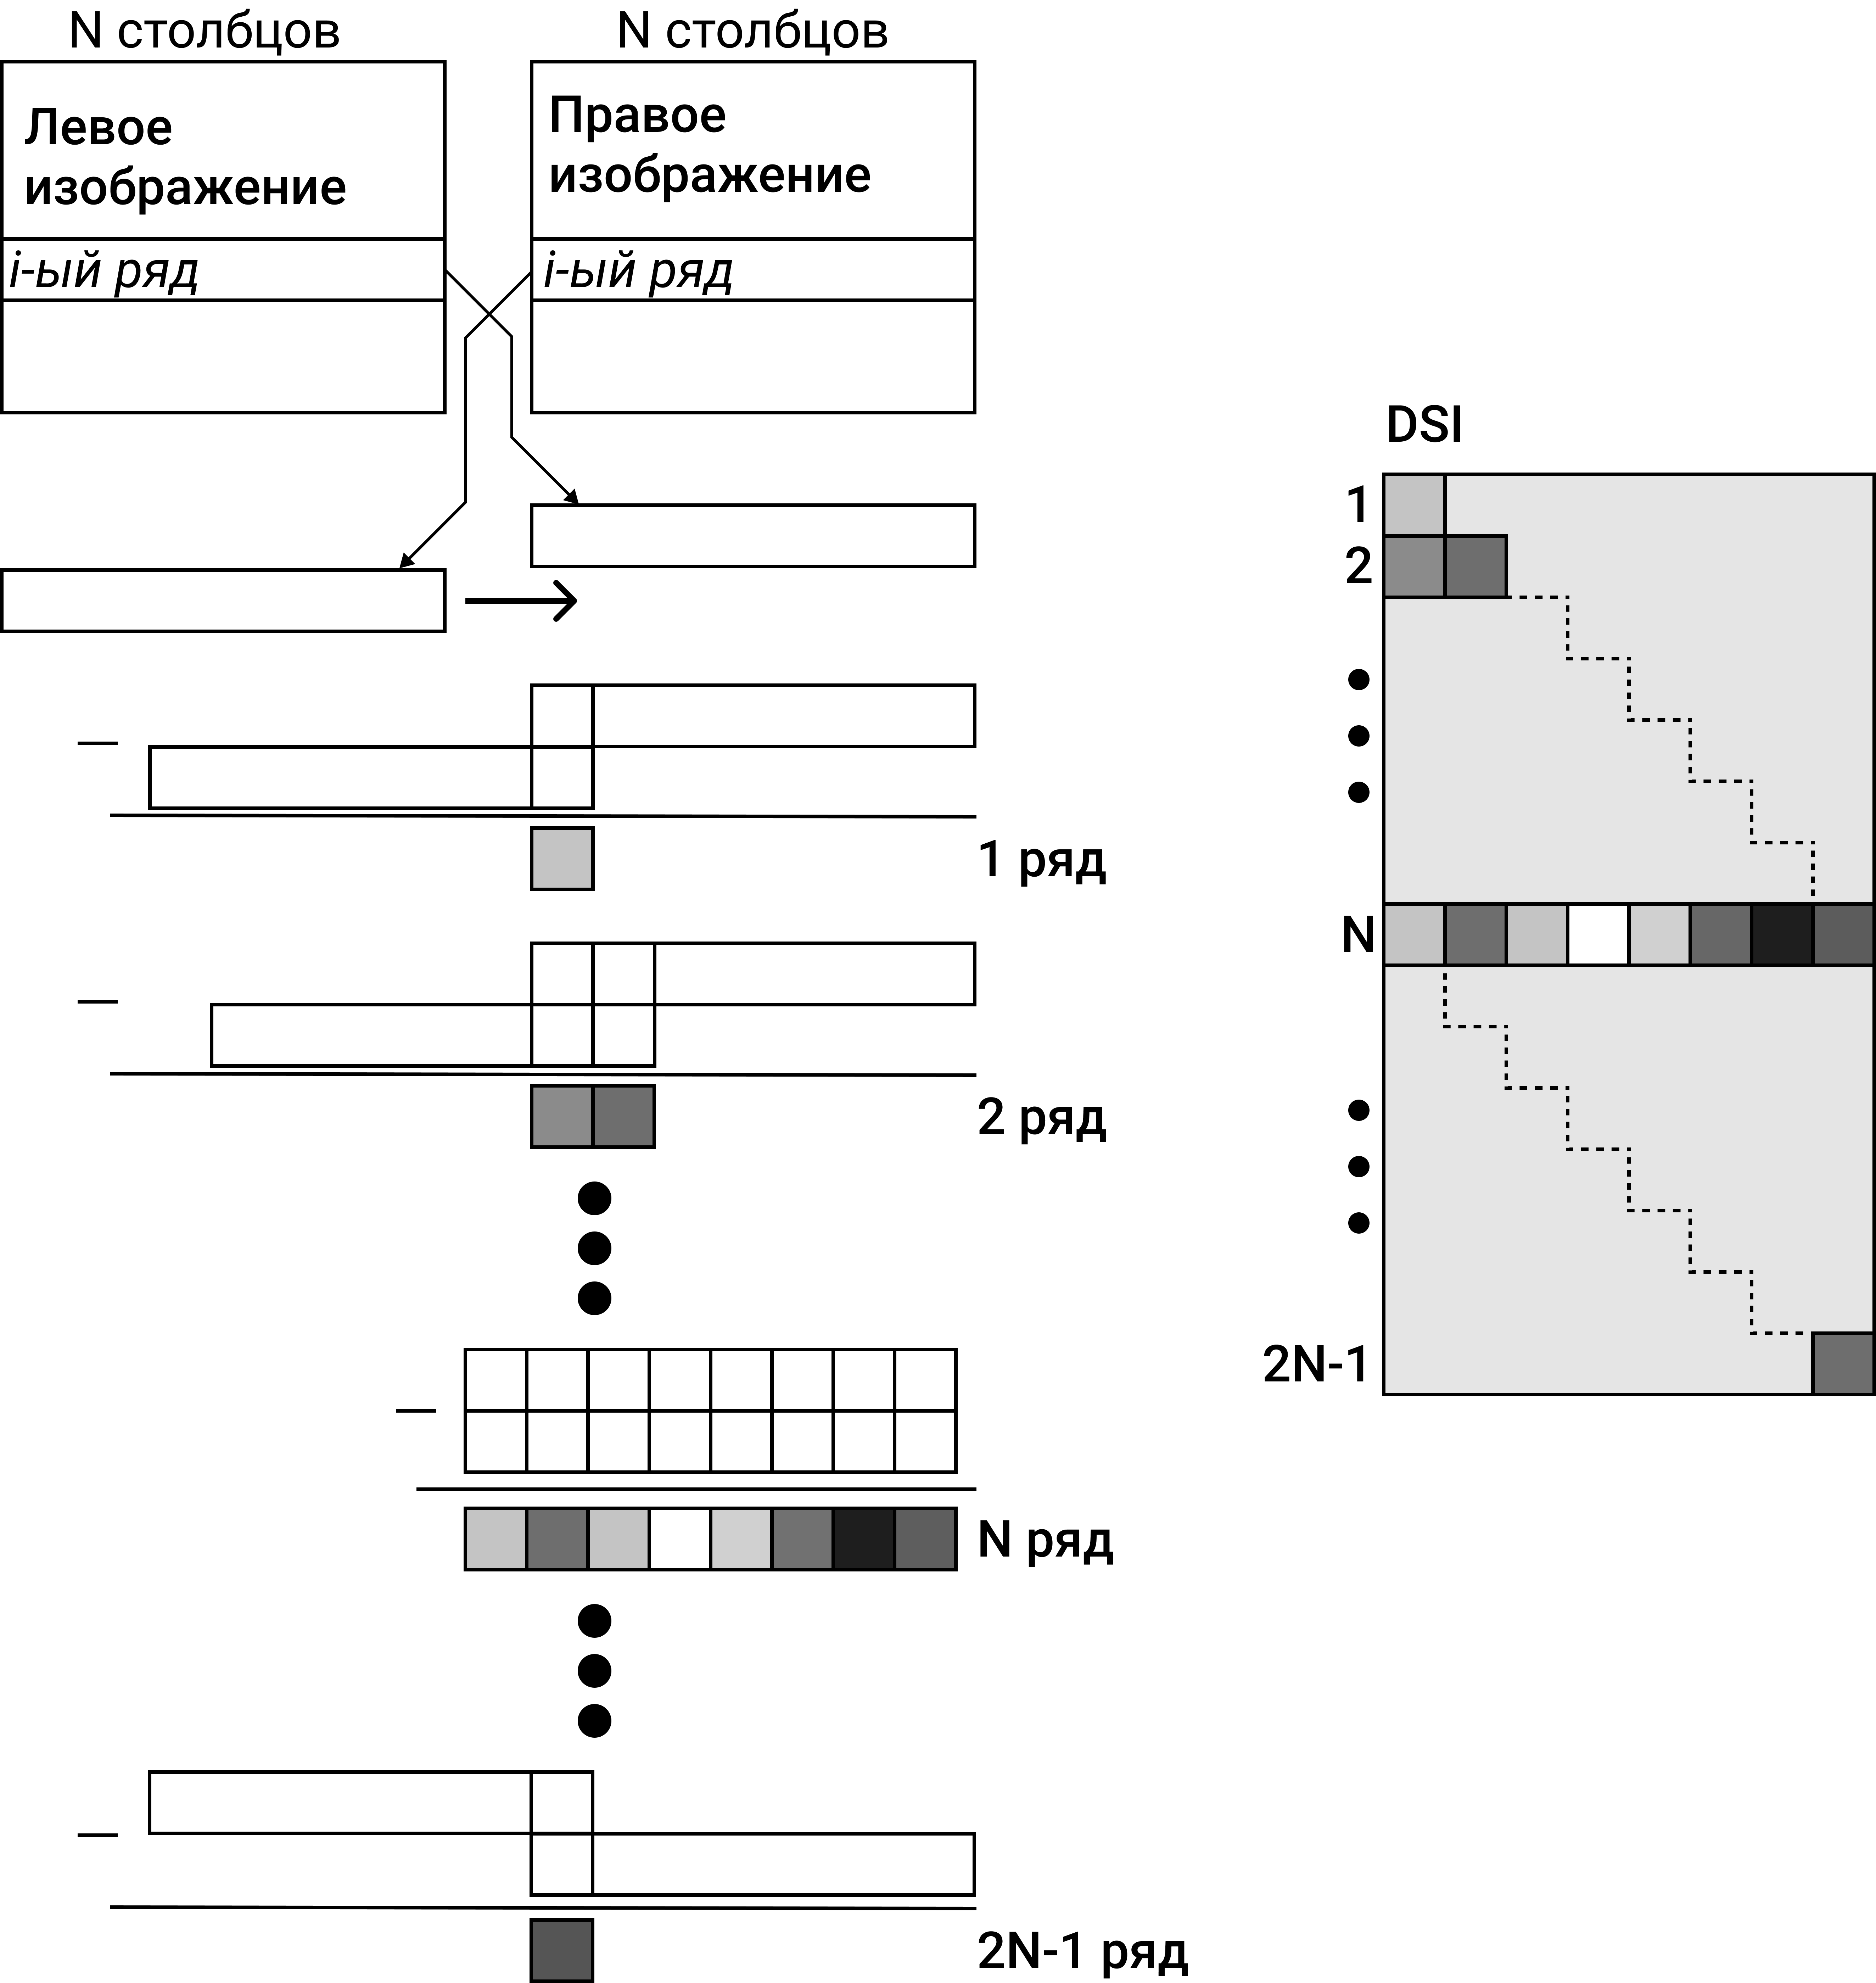
\includegraphics[scale=0.04]{pics/DSI_rus.png}
		\caption{Процесс построения DSI. Строка левого изображения считается неподвижной, пока строка правого изображения смещается вдоль неё. Результат вычитания 
				 перекрывающихся пикселей складывается в очередную строку DSI. Сам DSI обрезается с учётом ограничений.	} 
		\label{pic:DSI} % название для ссылок внутри кода
	\end{center}
\end{figure}
Далее задача состоит в поиске оптимального пути от левого верхнего угла до правого нижнего на полученной матрице. Для каждого элемента матрицы возможны три типа "движения": горизонтальный (означающий совпадение),
 вертикальный и диагональный (оба соответствуют заслонённым областям). Определяется тип движения по значению DSI в точке. Тем не менее, количество путей, которые можно построить, даже с этими ограничениями 
 остаётся довольно большим.

 Как уже упоминалось, динамическое программирование уменьшает вычислительную сложность задачи оптимизации   за счёт разбиения её на множество более простых и мелких задач. 
При применении к этой задаче это означает присвоение каждому элементу DSI стоимости, зависящей от доступного типа движения, и поиск оптимального пути от левого верхнего угла 
матрицы до правого нижнего. Поиск при этом опирается на расставленные ранее стоимости для выбора следующего шага пути. 

Данный алгоритм позволяет обрабатывать каждую строку изображения независимо и выполнять вычисления параллельно. Другими преимуществами является лучшее распознавание в слаботекстурированных 
областях по сравнению с локальными методами и возможность обработки заслонённых областей.   % % TODO: какой обработки? 
К недостаткам метода относят высокую вычислительную сложность (до $O(n^2)$) и возможность распространения локальной ошибки на последующие пиксели, что приводит к характерным горизонтальным полосам на картах глубины. 

Высокий интерес к этому методу привёл к появлению большого числа работ, пытающихся устранить недостатки метода и повысить его эффективность. Так была предложена модель \cite{symmetric}, которая 
опирается на ограничение видимости - предположение, что каждый заслонённый пиксель не имеет соответствия на втором изображении, а незаслонённый - обязательно имеет. В результате карты глубины не теряют информацию о глубине 
в местах, которые видит только одна камера, но при этом страдает детализация (рис. \ref{pic:symmetry}). 
\begin{figure}[H]
	\begin{center}
		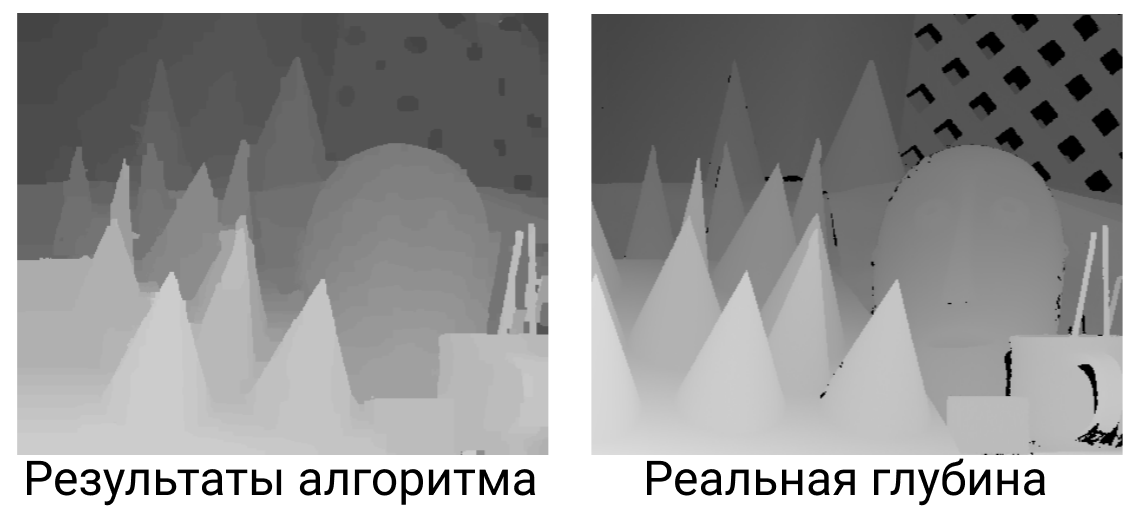
\includegraphics[scale=0.3]{pics/symmetric_rus.png}
		\caption{ Сравнение карты глубины, полученной алгоритмом, с эталонным изображением. } 
		\label{pic:symmetry} % название для ссылок внутри кода
	\end{center}
\end{figure}
Дополнительное ограничение, позволяющее уменьшить количество доступных путей, может дать использование заранее известных GCP (Ground Control Points). Эти точки, положение и 
соответствие которых можно определить заранее с большой точностью. Их использование позволяет снизить сложность поиска пути до 25\% от оригинальной задачи \cite{DSI}. 

\subsection{Алгоритм разреза графа}
Однако у предыдущего метода есть недостаток, выраженный в неспособности учитывать горизонтальные и вертикальные ограничения непрерывности. Эффективно исправить это в рамках динамического 
программирования пока не удалось. Альтернативный подход предлагает привести задачу к поиску максимального потока в графе. Для этого может использоваться случайное поле Маркова (MRF) - граф с вершинами, 
соответствующими пикселям левого изображения и рёбрами, отражающими зависимость между пикселями. Каждый пиксель имеет свою стоимость аналогично методу динамического программирования, а каждое рёбро - пропускную способность, 
зависящую от стоимости соединяемых им пикселей. Таким образом, граф выглядит как сетка, в которой каждая переменная (пиксель) зависит только от своих соседей, и задачу стереозрения можно переформулировать в терминах MRF.  
Для этого могут использоваться известные алгоритмы минимизации энергии на случайных полях Маркова. Карта расхождений по этому методу находится как плоскость, формирующая разрез представленного графа на две части с минимальной 
суммарной стоимостью входящих в него рёбер. Особенности построения и математическая формализация этих структур приведены в \cite{graphcut,gc_ocl}. 

Очевидно, что классические методы, основанные на алгоритме разреза графа, требуют больше вычислительных операций, чем даже динамическое программирование. Были предприняты попытки ускорить метод \cite{fast_gc,graphcut}, 
которые приблизили его по эффективности к динамическому программированию. Помимо вычислительных ресурсов алгоритм так же довольно требователен к памяти (до  150 раз больше объёма одного изображения), что осложняет его использование 
с большими изображениями, но и эта проблема решается применением более эффективных структур данных \cite{effic_gc}. Однако такая модификация алгоритма показывает результаты в среднем лишь на 1.6\%  лучше, чем ДП. 

Современные алгоритмы разреза графа являются одними из самых точных, но и самых медленных алгоритмов стереозрения.

\subsection{Алгоритмы на нейронных сетях}

Рост доступного объёма памяти в графических ускорителях и популярности алгоритмов, построенных с использованием неиросетей, а также возникновение качественных датасетов позволили реализовать надёжные и быстрые способы 
получения карт глубины, опирающиеся на глубокое обучение \cite{neural_review}. В настоящий момент существенная доля самых точных алгоритмов в популярном бенчмарке Middlebury Stereo Evaluation \cite{stereo_bench} представлена именно
подобными решениями. 

При  этом возможно применение нескольких подходов. Свёрточные нейронные сети могут выполнять лишь один этап классического метода стереозрения, например, поиск соответствий в эпиполярной линии \cite{cnn_match}. Более поздние работы 
экспериментировали с архитектурой сети, добиваясь, например, подсчёта стоимости сопоставления для каждого возможного расхождении \cite{cnn_improv}.  К этому же подходу относится использование неиронных сетей для постобработки 
карт глубины \cite{cnn_post1}.  
Второй подход подразумевает решение всей задачи получения карты глубины без необходимости в пост-обработке с помощью глубокого обучения. DispNetC \cite{cnn_ete1}, например, подсчитывает объём корреляции между особенностями двух изображений и использует свёрточную неиронную сеть 
для прямой регрессии карт расхождений, а GC-Net \cite{gc_net} впервые содержала модуль 3D-свёртки, который позже стал основой для более быстрых и точных алгоритмов.   

Таким образом, современные алгоритмы на глубоком обучении позволяют оценивать глубину по паре изображений с высокой точностью и производительностью в реальном времени для некоторых алгоритмов. Тем не менее их использование затруднено 
необходимостью использования современных графических ускорителей. 


\section{Выводы}
\label{conclusion}

Задача 3D-реконструкции остаётся активным полем работы для исследователей, занимающихся техническим зрением. В этой работе были представлены основные алгоритмы, применяемые на данный момент. По изученной литературе видно, что за последние два десятилетия  
фокус сместился с фундаментальных основ стереозрения к более частным исследованиям, направленным на повышение качества и скорости получения результатов, а также проблемным областям вроде обработки заслонений и слаботекстурированных регионов. Использование неиросетей 
для данной задачи также привело к появлению нового весьма перспективного класса алгоритмов. В настоящий момент присутствует запрос на эффективные методы стереозрения, способные работать в реальном времени и на мобильных платформах, удовлетворению 
этого запроса, вероятно, и будут посвящены дальнейшие исследования на эту тему. 



\newpage
\bibliographystyle{./config/splncs04}
\bibliography{refs}

\end{document}
